\documentclass[border=4pt]{standalone}
\usepackage{amsmath,amssymb,tikz}\usetikzlibrary{arrows.meta}
\definecolor{figB}{RGB}{31,90,166}\definecolor{figR}{RGB}{176,48,48}\definecolor{figG}{RGB}{46,125,50}\definecolor{figO}{RGB}{214,120,20}
\begin{document}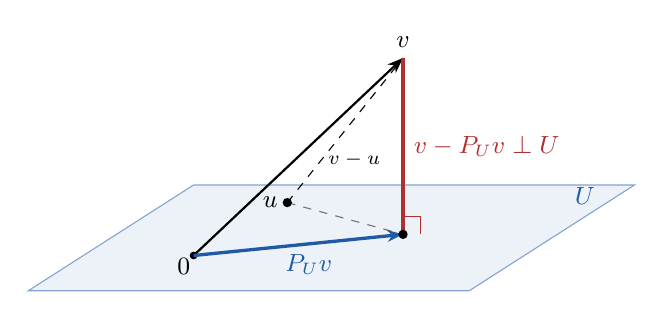
\begin{tikzpicture}[scale=1.4,>={Stealth[length=2mm]},x={(1cm,0cm)},y={(0.5cm,0.32cm)},z={(0cm,1cm)}]
\fill[figB!8] (-1,-1,0)--(3,-1,0)--(3,2,0)--(-1,2,0)--cycle; \draw[figB!55] (-1,-1,0)--(3,-1,0)--(3,2,0)--(-1,2,0)--cycle;
\node[figB,font=\small] at (2.7,1.7,0) {$U$};
\coordinate (O) at (0,0,0); \coordinate (P) at (1.6,0.6,0); \coordinate (Vv) at (1.6,0.6,1.6); \coordinate (Q) at (0.1,1.5,0);
\draw[dashed,black!55] (Q)--(P);
\draw[dashed,black] (Q)--(Vv) node[pos=0.3,right,font=\scriptsize,inner sep=2pt]{$v-u$};
\fill (O) circle (1pt) node[below left,font=\small,inner sep=1pt]{$0$};
\draw[->,thick] (O)--(Vv) node[above,font=\small]{$v$};
\draw[->,very thick,figB] (O)--(P) node[pos=0.55,below,font=\small]{$P_Uv$};
\draw[figR] (1.6,0.6,0.16)--++(0.16,0,0)--++(0,0,-0.16);
\draw[very thick,figR] (P)--(Vv) node[midway,right,font=\small]{$v-P_Uv\perp U$};
\fill (Q) circle (1.2pt) node[left,font=\small]{$u$};
\fill (P) circle (1.2pt);
\end{tikzpicture}\end{document}
